%!TEX root=../document.tex

\section{Ergebnisse}
\label{sec:Ergebnisse}
Es wurde entschieden eine Applikation mittels \verb|React Native| und \verb|Firebase| zu schreiben. Für die Datenspeicherung, Datenverwaltung und Datensynchronisation wurde die Cloud Datenbank \verb|Cloud Firestore| verwendet. 
\subsection{Anforderungen}
Es waren bestimmte Anforderungen gegeben, welche von der verwendeten Architektur bzw. Technologie erfüllt werden mussten: 
\begin{itemize}
	\item Daten speichern
	\item Daten lesen
	\item Daten ändern
	\item Daten löschen
	\item Daten synchronisieren
	\item Öffentlich ansprechbar
\end{itemize}
\subsection{Firebase}
Firebase ist eine Plattform entwickelt von Google welche eine Vielzahl von Features anbietet, hauptsächlich für mobile Applikation, namentlich Android und iOS. Firebase bietet eine Grundlage für viele technische Anforderungen und macht es auch möglich nach dem Release auf Nutzer einzugehen mittels diversen Analysetools, gezielten Werbungen, etc.. \cite{Firebase64:online}

\subsubsection{Cloud Firestore}
\textbf{Cloude Firestore} ist eine der vielen Features welche angeboten werden. Cloud Firestore ist eine flexible, skalierbare NoSQL Datenbank welche in der cloud agiert und es ermöglicht Daten zwischen Server und Client zu synchronisieren.\cite{CloudFir66:online}

Hierbei wurde zwischen Cloud Firestore und Realtime Database entschieden. Beide Produkte lösen das Problem der echtzeitigen Datensynchronisierung. Der große Unterschied ist jedoch wie Daten gespeichert werden. Während Realtime Database die Daten in einem großen JSON Objekt speichert, werden in Cloud Firestore Daten in Dokumenten abgespeichert. Dadurch ist es leichter Daten in besonders großen Projekten zu organisieren und es ist leichter zu skalieren.

Weiters ist es mit Cloud Firestore möglich die Applikation als Webservice anzubieten und es werden indexierte Queries verwendet um die Performance zu erhöhen.

Der große Nachteil and Cloud Firestore ist, dass das Produkt noch immer in der Beta-Phase ist. Somit ist Realtime Database stabiler und verlässlicher. Da dieses kleine Demoprojekt allerdings nicht 100\% zuverlässig sein muss, wurde Cloud Firestore verwendet um sich mit der Zukunft von Cloud-Datenspeicherung auseinanderzusetzen. \cite{ChooseaD34:online}
\subsubsection{Datenmodell}
Wie bereits erwähnt ist Cloud Firestore keine herkömmliche SQL Datenbank mit Spalten und Reihen. Stattdessen werden die Daten in \verb|documents| abgespeichert. Diese \verb|documents| werden weiterführend in \verb|collections| organisiert.

Jedes \verb|document| enthält eine beliebige Anzahl an \verb|key-value| Paaren. Es ist vergleichbar mit dem Aufbau und der Anwendung von JSON-Objekten.\cite{CloudFir12:online} 

\paragraph{Documents} 
Ist die \glqq Einheit\grqq\ der Speicherung in Cloud Firestore. Ein Dokument welches ein Shopping-Artikel enthält ist folgendermaßen aufgebaut:

\begin{lstlisting}[language=java]
	bought : false
	title : "Cookies"
\end{lstlisting}

Es ist allerdings, wie in JSON, auch möglich verschachtelte Attribute zu definieren:

\begin{lstlisting}[language=java]
	bought : false
	title :
		product: "Cookies"
		company : "Milka"
\end{lstlisting}

\cite[Abs. Documents]{CloudFir12:online}
\paragraph{Collections}
Sind als \glqq Container\grqq\ für die einzelnen \verb|documents| zu verstehen. Somit ist es leichter diese zu organisieren und zu verwalten. Im Beispiel der Einkaufliste, werden die einzelnen Artikel in Einkauflisten organisiert, wobei eine Einkaufsliste eine \verb|collection| darstellt. \cite[Abs. Collections]{CloudFir12:online}
\subsubsection{Synchronisation}
Um Echtzeit-Synchronisation zu ermöglichen wird eine Funktion bereitgestellt welche aufgerufen wird sobald eine Änderung in der Datenbank, \verb|collection| oder \verb|document| auftritt, \verb|onSnapshot()|. Hierbei ist wichtig das entschieden kann auf was genau gehört werden soll. Wenn nur eine bestimmte \verb|collection| oder sogar nur ein \verb|document| von Interesse ist, kann mit \verb|onSnapshot()| nur auf Änderungen dieser Objekte gehorcht werden. Beim ersten Aufruf wird ein gesamter Snapshot des angefragten Objektes mitgeliefert, bei weiteren Änderungen werden nur mehr die Änderungen mitgeliefert um die Performance zu verbessern. 

Durch folgenden Code kann auf Änderungen der Einkaufliste gehorcht werden:

\begin{lstlisting}[language=java]
	// Referenz in einer Variable speichern
	this.ref = firebase.firestore().collection('shoppinglist');
	// onSnapshot liefert automatisch eine Funktion zurueck welche aufgerufen werden kann um sich von Updates "abzumelden"
	this.unsubscribe = this.ref.onSnapshot(this.onCollectionUpdate.bind(this))
\end{lstlisting}
\clearpage
\subsubsection{Schnittstellen}
Die wichtigsten Schnittstellen in Cloud Firestore sind folgende\cite{Interfac64:online}:

\begin{itemize}
	\item \textbf{app} (firebase.firestore.app)
	
	Ist die Applikation welcher mit dieser Firestore Instanz assoziiert ist
	\item \textbf{batch()} (firebase.firestore.WriteBatch)
	
	Mit dieser Funktion können mehrere Einträge auf einmal in die Datenbank geschrieben werden
	\item \textbf{collection()} (firebase.firestore.CollectionReference)
	
	Diese Funktion liefert die Referenz der als Parameter angegeben \verb|collection| zurück. Ist die wahrscheinlich wichtigste Funktion, da mit der Referenz Dokumente geschrieben, gelöscht und verwaltet werden können.
	\item \textbf{doc()} (firebase.firestore.DocumentReference)
	
	Diese Funktion liefert die Referenz des als Parameter angegebenen \verb|documents| zurück. Somit können nur einzelne Dokumente bearbeitet werden. 
\end{itemize}
\subsection{Alternative Technologien}

\begin{itemize}
	\item \textbf{Couchbase Mobile}
	
	Ist ebenfalls eine NoSQL Datenbank welche es ermöglicht Daten zwischen mobilen Applikation auszutauschen. \cite{Couchbas67:online}
	\item \textbf{Deployd}
	
	Verspricht eine Open-Source Alternative zu Firebase darzustellen \cite{deployd58:online}. Deployd hat allerdings nicht annähernd das breitgefächerte Arsenal an Features und kaum Community support. 
	\item \textbf{Firehose}
	
	Ist ein minimalistischer Ansatz um Clients und Server synchron zu halten wie Websockets. \cite{Firehose82:online}
	\item \textbf{\glqq Händisch\grqq\ mit Websockets}
	
	Natürlich ist es auch möglich selber einen Node Server aufzusetzen und auf diesen alle Clients mit Websockets zu verwalten. 
\end{itemize}

\subsection{Umsetzung}
\subsubsection{Projekt aufsetzen}
Um das Projekt aufzusetzen wurde das Projekt \href{https://github.com/invertase/react-native-firebase-starter}{react-native-firebaser-starter} als Basis verwendet. Dieses enthält zusätzlich ein Tutorial \cite{invertas82:online} welches verwendet wurde um die Applikation korrekt aufzusetzen.

Der erste Schritt war es im Basisprojekt alle nötigen Dependencies (\verb|node_modules/|) zu installieren mittels \verb|npm install|. Der nächste Schritt war es das Projekt einen Namen zu geben. Dafür gibt es ein Script welches mittels \verb|npm run rename| ausgeführt wird, anschließend wird nach Name und Organisation gefragt und man erhält folgende Ausgabe:

\begin{minipage}{\linewidth}
	\centering
	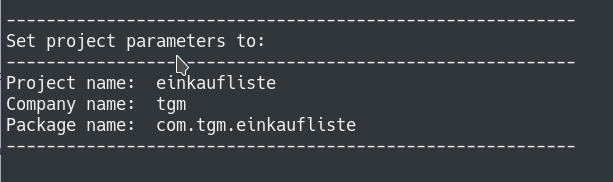
\includegraphics[width=0.8\linewidth]{images/1}
	\figcaption{Projektparameter wurden angegeben}
\end{minipage}
\subsubsection{Firebase Projekt anlegen}
Der nächste Schritt war es mit den angelegten Daten ein Firebase Projekt anzulegen und anschließend auszuwählen dass Firebase zu der Applikation hinzugefügt werden soll. Hierbei muss der Packagename angegeben werden, welcher im vorigen Schritt durch Angabe von Name und Organisation definiert wurde. Zusätzlich ist noch möglich ein Nickname und ein Signaturzertifikat anzugeben. 

\begin{minipage}{\linewidth}
	\centering
	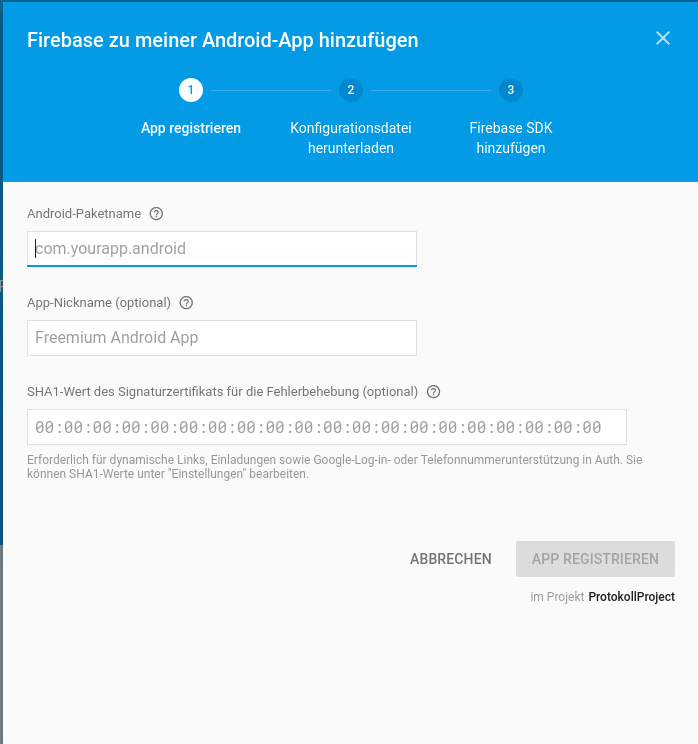
\includegraphics[width=0.7\linewidth]{images/2}
	\figcaption{Firebase dem Projekt hinzufügen}
\end{minipage}
Im nächsten Schritt kann nun ein Konfigurationsfile heruntergeladen werden, \verb|google-services.json|, dieses muss anschließend im Ordner \verb|android/app/| gespeichert werden. 

Falls man alles richtig gemacht hat sollte es nun möglich sein die Demoapplikation auszuführen mit \verb|react-native start| und \verb|react-native run-android|. Man sollte mit einem Logo, Text und allen aktivierten Firebase Modulen begrüßt werden.
\subsubsection{Daten einfügen}
Wie bereits beschrieben, wurde zuerst eine Referenz auf die \verb|shoppinglist|-Collection erstellt. Mit dieser Referenz können Daten hinzugefügt werden. Beim drücken des Submit-Buttons, wird die Funktion \verb|addItem()| aufgerufen, welche mittels der Referenz und dem Text welcher eingegeben wurde ein neues Dokument anlegt:

\begin{lstlisting}[language=java]
this.ref.add({
	title: this.state.textInput,
	bought: false,
});
\end{lstlisting}

\clearpage
Nach Hinzufügen eines Artikels kann nun auf der Firebase Konsole \cite{Firebase65:online} eingesehen werden, ob tatsächlich in der Collection ein neues Dokument angelegt wurde:

\begin{minipage}{\linewidth}
	\centering
	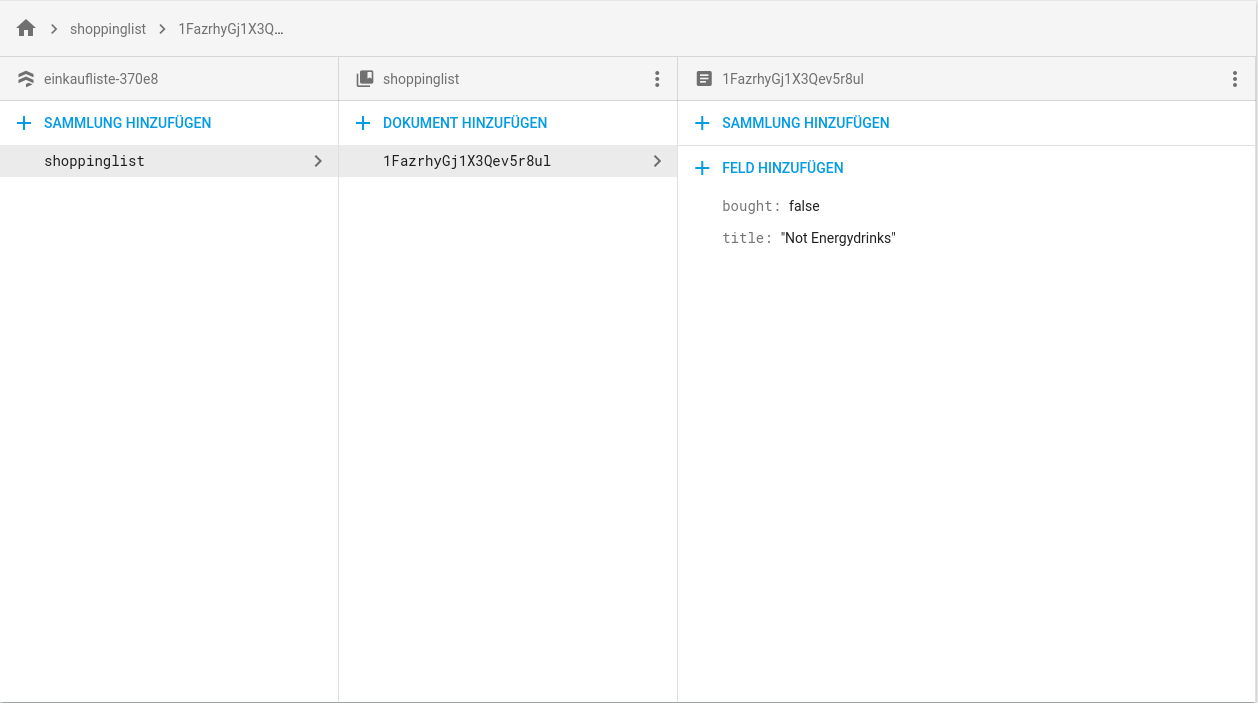
\includegraphics[width=1\linewidth]{images/3}
	\figcaption{Der Collection wurde ein neues Dokument hinzugefügt}
\end{minipage}
\subsubsection{Daten anzeigen}
Die Daten werden in einer \verb|FlatList| angezeigt. Mit der Flatlist ist es möglich, ein Array an Daten anzugeben welches angezeigt werden soll, und zu definieren wie jedes einzelner dieser Elemente gerendered werden soll in der Liste. Um jeden Artikel darzustellen wurde ein Component \verb|ShoppingItem| geschrieben, welches das \verb|item| der Liste entgegennimmt.

\begin{lstlisting}[language=java]
<FlatList
	data={this.state.shoppingList}
	renderItem={({item}) => 
		<ShoppingItem item={item}/> 
	}
>
\end{lstlisting}
ShoppingItem ist ein \verb|touchable|, wenn einmal gedrückt wird, wird indiziert dass der Artikel gekauft wurde, bei langem Drücken wird der Artikel aus der Liste gelöscht. 

\subsubsection{Daten auslesen}
Um Daten auszulesen wird eine Callbacke Methode \verb|onCollectionUpdate()| definiert, welche aufgerufen wird sobald \verb|onSnapshot()| gefeuert wird. \verb|onCollectionUpdate()| nimmt einen Snapshot als Parameter, iteriert diesen um die alte Liste mit der neuen zu ersetzen. Wie bereits erwähnt, wird nur beim ersten Aufruf der gesamte Snapshot der Collection iteriert, nach jedem weiteren Aufruf werden nur mehr die Änderungen verarbeitet. 

Um die interne Speicherung zu erleichtern, wird zusätzlich zum Inhalt jedes Dokuments in einer Liste noch das gesamte Dokument und eine eindeutig identifizierbarer Schlüssel gespeichert:

\begin{lstlisting}[language=java]
	snap.forEach((el) => {
		let { title, bought} = el.data()
		let key : number = el.id
		shoppingList.push({
			key: key,
			doc: el,
			title,
			bought
		});
	});
\end{lstlisting}
\subsubsection{Daten löschen}
Wie bereits erwähnt, wird beim langen Drücken eines ShoppingItems der Artikel gelöscht. Dafür wurde im ShoppingItem die Funktion \verb|delete()| geschrieben, welche das gesamte Dokument, welches als Prop an die Komponente übergeben wurde, löscht:

\begin{lstlisting}[language=java]
delete() {
	this.props.item.doc.ref.delete()
}
\end{lstlisting}
\subsubsection{Daten ändern}
Um zu indizieren dass ein Artikel gekauft wurde, wurde das Attribut \verb|bought| im Dokument definiert. Beim einmaligen Drücken eines Artikels, wird die Funktion \verb|toggleBought()| aufgerufen. Diese setzt das Attribut \verb|bought| in der Datenbank auf das Gegenteil welches es davor war:

\begin{lstlisting}[language=java]
this.props.item.doc.ref.update({
	bought: !this.props.item.bought,
});
\end{lstlisting}

Zusätzlich wurde noch eine Animation hinzugefügt. Diese Animation lässt einen Artikel innerhalb von 500 Millisekunden Grün erscheinen, sobald dieser gekauft wurde. Falls er, aus welchem Gründen auch immer, doch nicht gekauft wurde, wechselt die Farbe wieder innerhalb von 500ms zu weiß zurück. Dies wurde mit dem \verb|Animated| Modul von React Native umgesetzt:

\begin{lstlisting}[language=java]
Animated.timing(this.animatedValue, {
	toValue: this.props.item.bought ? 0 : 150,
	duration: 500
}).start()
\end{lstlisting}
\subsubsection{Replikation zur Konsistenzwahrung}
Dadurch dass Cloud Firestore die Infrastruktur der Google Cloud Platform verwendet, werden die Daten über mehrere Regionen repliziert und starke Konsistenz-Garantie ist gegeben.\cite[Abs. Key capabilities]{CloudFir66:online}
\subsubsection{Offline-Verfügbarkeit}
Offline Verfügbarkeit ist automatisch in Cloud Firestore aktiviert. Hierbei wird eine gecachede Kopie der Daten auf dem Gerät gespeichert. Diese Daten können offline geändert werden und wenn das Gerät wieder online ist, werden diese Daten synchronisiert.  \cite{EnableOf96:online}
\subsubsection{Öffentlich ansprechbar}
Dadurch dass es ein Google Service ist, ist Cloud Firestore öffentlich ansprechbar.
\subsubsection{Kosten}
Der Service ist gratis ist jedoch folgendermaßen limitiert:


\begin{minipage}{\linewidth}
	\centering
	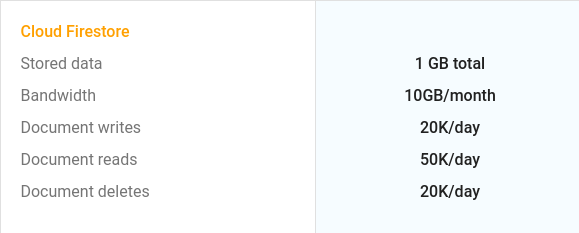
\includegraphics[width=0.7\linewidth]{images/4}
	\figcaption{Limitierungen bei der Gratis-Version von Firebase}
\end{minipage}

